\documentclass[10pt, landscape]{article}
\usepackage[scaled=0.92]{helvet}
\usepackage{calc}
\usepackage{multicol}
\usepackage[a4paper,margin=3mm,landscape]{geometry}
\usepackage{amsmath,amsthm,amsfonts,amssymb}
\usepackage{color,graphicx,overpic}
\usepackage{hyperref}
\usepackage{newtxtext} 
\usepackage{enumitem}
\usepackage[table]{xcolor}
\usepackage{mathtools}
\setlist{nosep}
% for including images
\graphicspath{ {./images/} }

\pdfinfo{
  /Title (MODULE_CODE.pdf)
  /Creator (TeX)
  /Producer (pdfTeX 1.40.0)
  /Author (Jovyn Tan)
  /Subject (MODULE_CODE)
/Keywords (MODULE_CODE, nus,cheatsheet,pdf)}

% Turn off header and footer
\pagestyle{empty}

% redefine section commands to use less space
\makeatletter
\renewcommand{\section}{\@startsection{section}{1}{0mm}%
  {-1ex plus -.5ex minus -.2ex}%
  {0.5ex plus .2ex}%x
{\normalfont\large\bfseries}}
\renewcommand{\subsection}{\@startsection{subsection}{2}{0mm}%
  {-1explus -.5ex minus -.2ex}%
  {0.5ex plus .2ex}%
{\normalfont\normalsize\bfseries}}
\renewcommand{\subsubsection}{\@startsection{subsubsection}{3}{0mm}%
  {-1ex plus -.5ex minus -.2ex}%
  {1ex plus .2ex}%
{\normalfont\small\bfseries}}%
\makeatother

\renewcommand{\familydefault}{\sfdefault}
\renewcommand\rmdefault{\sfdefault}
%  makes nested numbering (e.g. 1.1.1, 1.1.2, etc)
\renewcommand{\labelenumii}{\theenumii}
\renewcommand{\theenumii}{\theenumi.\arabic{enumii}.}
\renewcommand\labelitemii{•}
\renewcommand\labelitemiii{•}

\definecolor{mathblue}{cmyk}{1,.72,0,.38}
\everymath\expandafter{\the\everymath \color{mathblue}}

% Don't print section numbers
\setcounter{secnumdepth}{0}

\setlength{\parindent}{0pt}
\setlength{\parskip}{0pt plus 0.5ex}
%% adjust spacing for all itemize/enumerate
\setlength{\leftmargini}{0.5cm}
\setlength{\leftmarginii}{0.5cm}
\setlist[itemize,1]{leftmargin=2mm,labelindent=1mm,labelsep=1mm}
\setlist[itemize,2]{leftmargin=4mm,labelindent=1mm,labelsep=1mm}

% adding my commands
% tightcenter
\newenvironment{tightcenter}{%
  \setlength\topsep{0pt}
  \setlength\parskip{0pt}
  \begin{center}
    }{%
  \end{center}
}

% boxed
\newenvironment{tightbox}{%
  \setlength\topsep{0pt}
  \setlength\parskip{0pt}
  \begin{center}
    \begin{tabular}{|@{\hspace{\dimexpr\fboxsep+0.5\arrayrulewidth}}c@{\hspace{\dimexpr\fboxsep+0.5\arrayrulewidth}}|}
      \hline
    }
    {%
    \\ \hline
    \end{tabular}
  \end{center}
}

% fixed width box
\newenvironment{fixedbox}[1][0.7]{
  \setlength\topsep{0pt}
  \setlength\parskip{0pt}
  \begin{center}
    \begin{tabular}{|>{\centering\arraybackslash}m{#1\linewidth}|}
    \hline
  }{
  \\ \hline
  \end{tabular}
  \end{center}
}

% definition of a new term
\usepackage{soul}
\definecolor{paleyellow}{RGB}{251,243,218}
\newcommand{\definition}[2][]{\sethlcolor{paleyellow}\hl{\textbf{#2}} #1  $\rightarrow$}

% important note (attention)
\newcommand{\attention}{{\color{red}\textbf{! }}}



% -----------------------------------------------------------------------

\begin{document}
\raggedright
\footnotesize
\begin{multicols*}{4}
  % multicol parameters
  \setlength{\columnseprule}{0.25pt}

  \begin{center}
    \fbox{%
      \parbox{0.8\linewidth}{\centering \textcolor{black}{
          {\Large\textbf{CS3236}}
        \\ \normalsize{AY22/23 SEM 1}}
        \\ {\footnotesize \textcolor{gray}{github/jovyntls}}
      }%
    }
  \end{center}

  \section{00. INTRODUCTION}

  \subsection{data compression}

  \begin{itemize}
    \item types of compression
      \begin{itemize}
        \item \textbf{lossless compression} - can recover the contents
        \item \textbf{lossy compression} - lose some quality - cannot convert back to the higher-quality version
      \end{itemize}
    \item examples
      \begin{itemize}
        \item sparse binary string - storing positions of 1s
        \item equal number of 0/1s - $L \geq \log_2 \binom{64}{32} \approx 60.7$
        \item english text - using relative frequency
        \item morse code is NOT binary (contains spaces)
      \end{itemize}
    \item info theory uses \textbf{probabilistic models} (letter frequency, sequence probabilities)
    \item 2 distinct approaches to compression:
      \begin{itemize}
        \item \textbf{variable length} - map more probable sequences to shorter binary strings
        \item \textbf{fixed length} - map most probable sequences to strings of a given length
          \begin{itemize}
            \item insufficient strings for low-probability sequences 
            \item tradeoff between length/failure probability
          \end{itemize}
      \end{itemize}
  \end{itemize}

  \subsection{information theory concepts}
  \begin{itemize}
    \item speed: \definition{rate} $\frac{k}{n}$ (mapping $k$ bits to $n$ bits)
    \item reliability: $ \mathbb{P}[error] $ = $\mathbb{P}[\text{estimated msg $\neq$ true msg}]$
    \item \definition{source coding theorem} the fundamental compression limit is given by a source-dependent quantity known as the \textbf{(Shannon) entropy $H$}. The (average) storage length can be arbitrarily close to $H$, but can never be any lower than $H$.
      \begin{itemize}
        \item $H$ is a property of the \textit{probability distribution}
      \end{itemize}
    \item \definition{channel coding theorem} there exists a channel-dependent quantity called the \textbf{(Shannon) capacity $C$} such that arbitrarily small error probability can be achieved only for rates $<C$
      \begin{itemize}
        \item can achieve $ \mathbb{P}[error] \leq \epsilon \iff$ rate $<C$
      \end{itemize}
  \end{itemize}

  \subsection{data communication example}

  \begin{itemize}
    \item a "transmitter" sends a sequence of 0s and 1s
    \item a "receiver" sends a sequence \textit{with some corruptions}
  \end{itemize}

  \subsubsection{channel transition diagram}

  \begin{minipage}[c]{0.3\linewidth}
    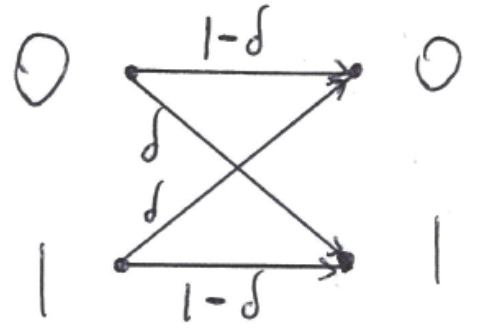
\includegraphics[width=0.8\linewidth]{cs3236-channel-transition-diagram.png} 
  \end{minipage}
  \begin{minipage}[c]{0.65\linewidth}
    \begin{itemize}
      \item each bit is flipped independently with probability $\delta \in (0, \frac{1}{2})$
    \end{itemize}
  \end{minipage}

  \subsubsection{naive}

  \begin{itemize}
    \item \textbf{uncoded communication} - $\mathbb{P}[correct] = (1-\delta)^N $
    \item \textbf{repetition code} - transmit "000" for "0", "111" for "1"
      \begin{itemize}
        \item $ \mathbb{P}[correct] = [(1-\delta)^3 + 3\delta(1-\delta)^2]^N $
        \item more reliable but 3x slower!
      \end{itemize}
  \end{itemize}

  \subsubsection{Hamming code}

  \begin{itemize}
    \item able to correct one bit flip
    \item maps binary string of length 4 to binary string of length 7
    \item fill in $b_1b_2b_3b_4$ and assign $c_1c_2c_3$ such that the sum of bits in each circle is even
      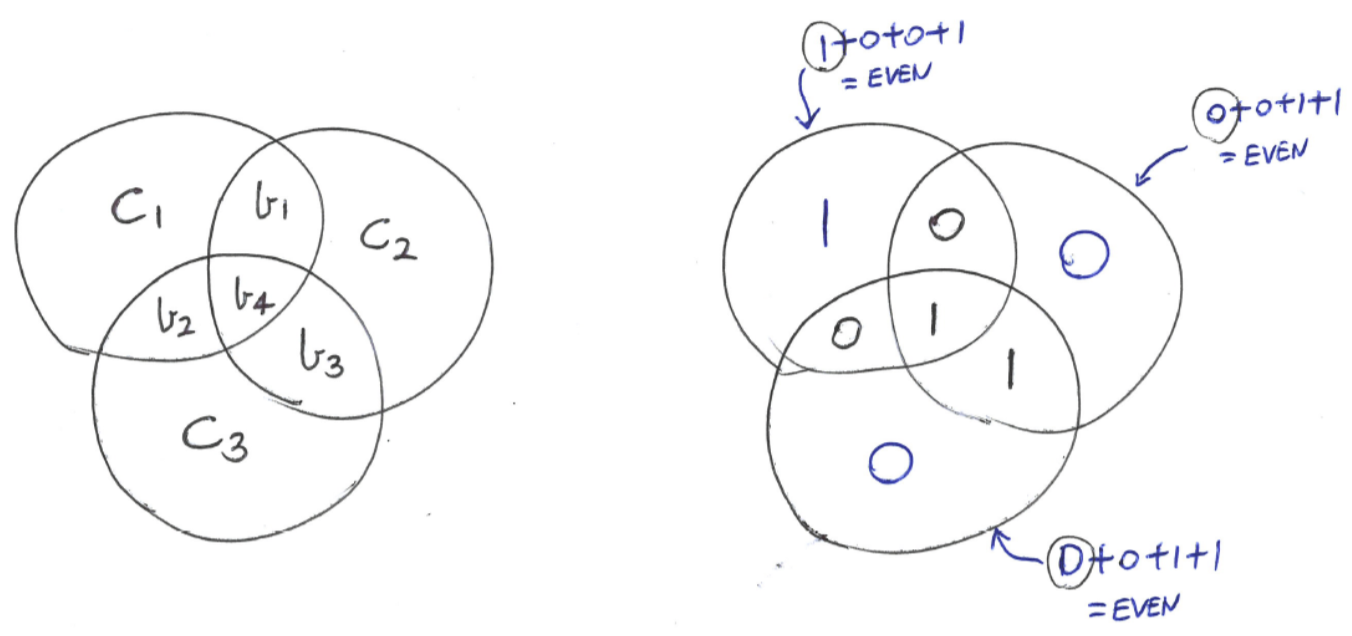
\includegraphics[width=0.9\linewidth]{cs3236-hamming-example.png} 
    \item $ \mathbb{P}[correct] \geq \mathbb{P}[\leq 1\text{bit flips}] = (1-\delta)^7 + 7\delta(1-\delta)^6 $
      \item with $\delta=1$: Shannon capacity $C\approx 0.531$ 
  \end{itemize}


\end{multicols*}

\end{document}
